\documentclass{article}

\usepackage{graphicx}
\usepackage{tikz}
\usepackage{tikzsymbols}
\usetikzlibrary{calc,patterns,shapes.geometric}
\pagestyle{empty}
\usepackage[margin=0pt]{geometry}
\geometry{papersize={14in,12in}}

\def\centerarc[#1](#2)(#3:#4:#5){\draw[#1] ($(#2)+({#5*cos(#3)},{#5*sin(#3)})$) arc (#3:#4:#5);}

\begin{document}
	\begin{figure}
		\centering
		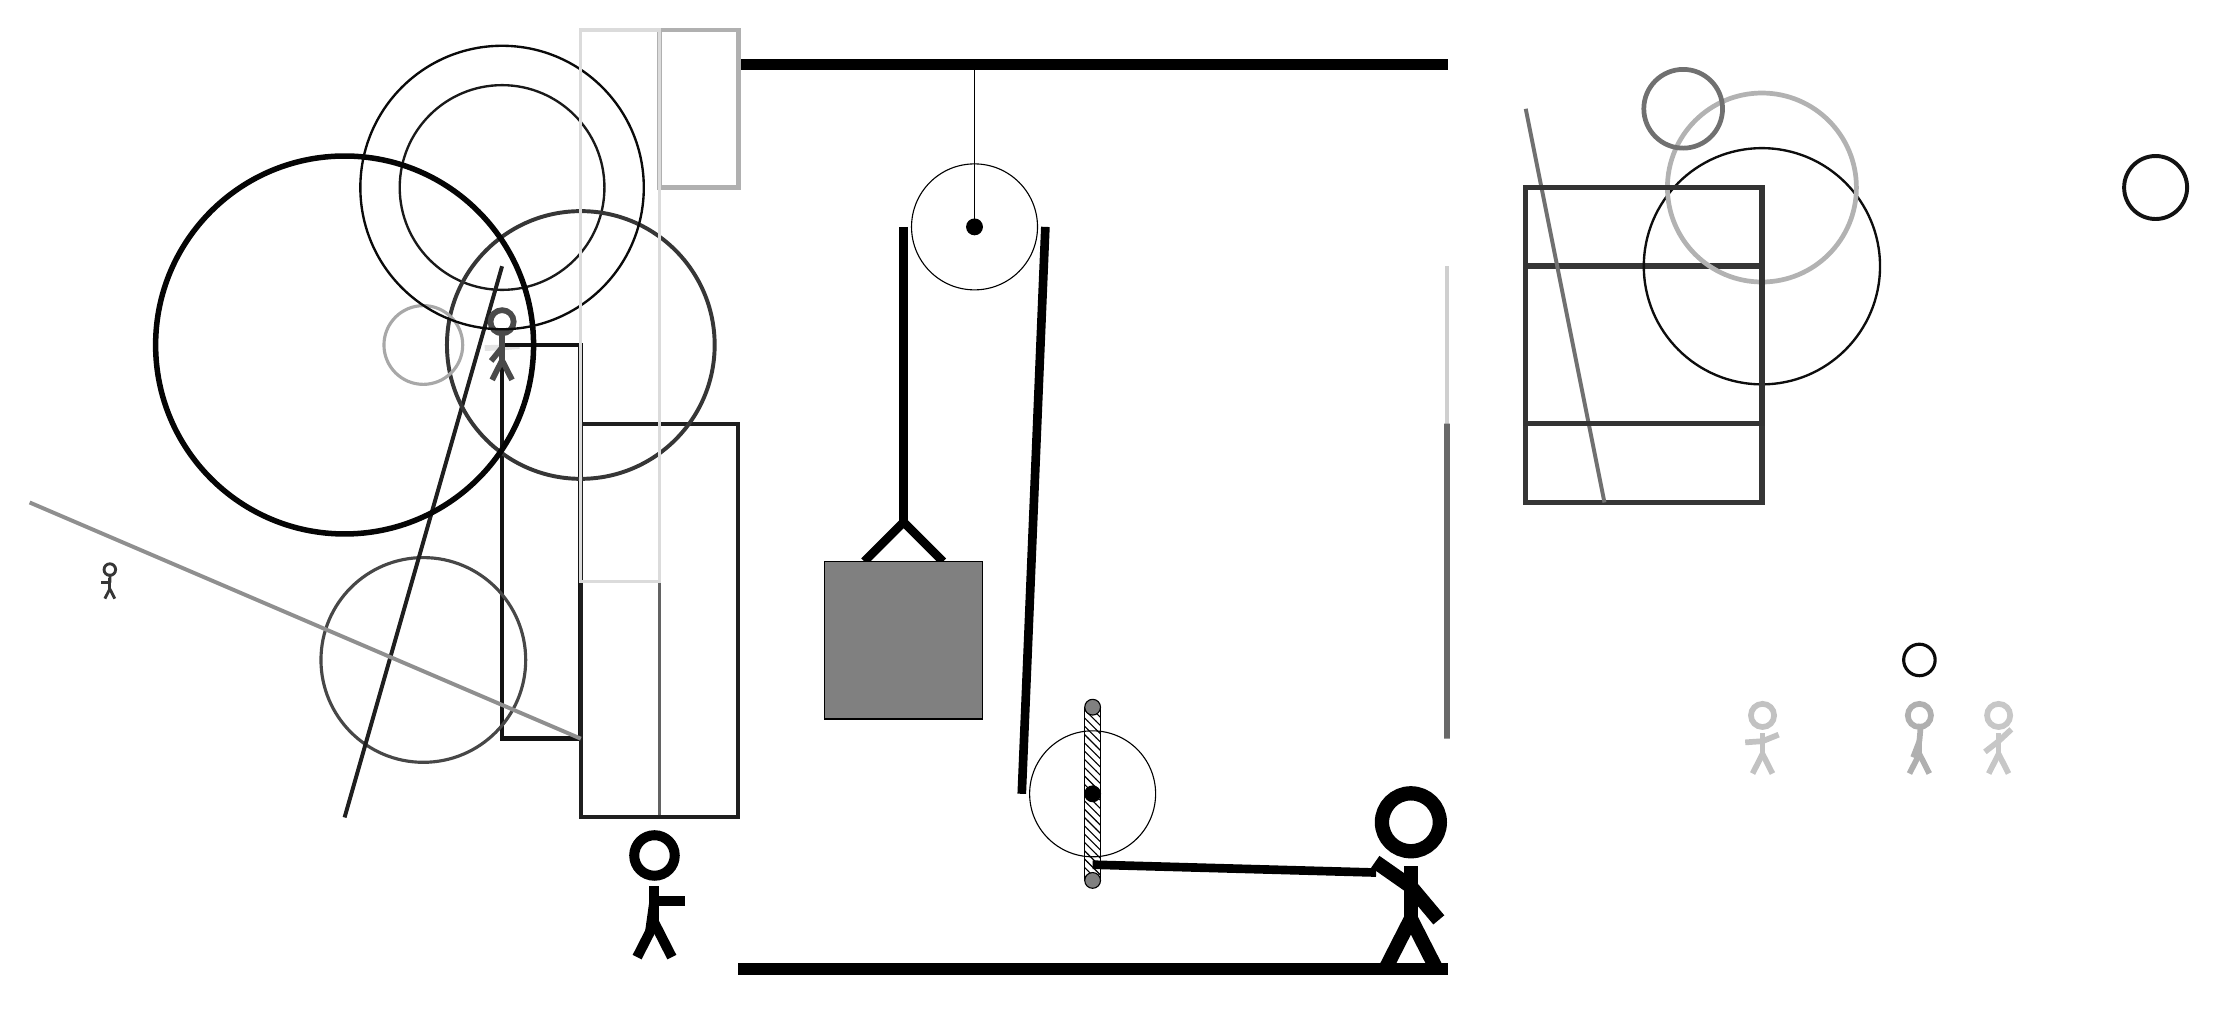
\begin{tikzpicture}
			%%%%% START %%%%%
			
			\draw[fill=black] (-2, 11.5) rectangle (7, 11.625);
			
			\draw (1, 9.5) circle (0.8);
			\draw[fill=black] (1, 9.5) circle (0.1);
			\draw (1, 11.5) -- (1, 9.5);
			
			\draw[fill=white](2.5, 2.3) circle (0.8);
			\draw[fill=black] (2.5, 2.3) circle (0.1);
			\draw[pattern=north west lines, pattern color=black] (2.4, 3.4) rectangle (2.6, 1.2);
			\draw[fill=black!50] (2.5, 3.4) circle (0.1);
			\draw[fill=black!50] (2.5, 1.2) circle (0.1);
			
			\draw[line width=1.1mm] (-0.4, 5.25) -- (0.1, 5.75) -- (0.6, 5.25);
			\draw[fill=black!50] (-0.9, 5.25) rectangle (1.1, 3.25);
			
			\draw[line width=1.1mm] (0.1, 9.5) -- (0.1, 5.75);
			\centerarc[line width=1.1mm](1, 9.5)(0:180:0.9);
			\draw[line width=1.1mm](1.9, 9.5) -- (1.6, 2.3);
			\centerarc[line width=1.1mm](2.5, 2.3)(180:270:0.9);
			\draw[line width=1.1mm](2.5, 1.4) -- (6.1, 1.3);
			
			\node[line width=0.7mm, color=black!11] at (-5, 8) {\Strichmaxerl[4][2][5]};
			
			\draw [line width=0.5mm, color=black!93](16, 10) circle (0.4);
			\draw[line width=0.5mm, color=black!94](11, 1) -- (11, 1);
			\draw[line width=0.6mm, color=black!93] (-4, 3) rectangle (-5, 8);
			
			\node[line width=0.3mm, color=black!31] at (13, 3) {\Strichmaxerl[4][69][85]};
			\draw [line width=0.3mm, color=black!90](-5, 10) circle (1.3);
			\draw[line width=0.4mm, color=black!61] (-3, 7) rectangle (-4, 2);
			\draw[line width=0.6mm, color=black!31] (-3, 12) rectangle (-2, 10);
			\node[line width=0.3mm, color=black!79] at (-10, 5) {\Strichmaxerl[2][0][88]};
			\draw[line width=0.7mm, color=black!79] (8, 6) rectangle (11, 9);
			\draw [line width=0.3mm, color=black!95](11, 9) circle (1.5);
			
			\draw [line width=0.4mm, color=black!72](-6, 4) circle (1.3);
			\draw[line width=0.5mm, color=black!19] (7, 9) rectangle (7, 5);
			
			\draw[line width=0.5mm, color=black!88] (-2, 7) rectangle (-4, 2);
			\draw[line width=0.5mm, color=black!88](-5, 9) -- (-7, 2);
			\draw[line width=0.5mm, color=black!44](-4, 3) -- (-11, 6);
			\node[line width=0.2mm, color=black!22] at (14, 3) {\Strichmaxerl[4][38][43]};
			
			\draw [line width=0.6mm, color=black!30](11, 10) circle (1.2);
			\draw[line width=0.5mm, color=black!56](8, 11) -- (9, 6);
			\node[line width=0.3mm, color=black!24] at (11, 3) {\Strichmaxerl[4][4][22]};
			\draw[line width=0.7mm, color=black!80] (8, 10) rectangle (11, 7);
			
			\draw [line width=0.4mm, color=black!96](13, 4) circle (0.2);
			\draw [line width=0.5mm, color=black!79](-4, 8) circle (1.7);
			\draw [line width=0.4mm, color=black!34](-6, 8) circle (0.5);
			\node[line width=0.7mm, color=black!100] at (-3, 1) {\Strichmaxerl[7][82][0]};
			
			\draw [line width=0.6mm, color=black!56](10, 11) circle (0.5);
			
			\draw[line width=0.7mm, color=black!59] (7, 7) rectangle (7, 3);
			\draw [line width=0.7mm, color=black!98](-7, 8) circle (2.4);
			
			\node[line width=0.6mm, color=black!71] at (-5, 8) {\Strichmaxerl[4][51][90]};
			\draw [line width=0.3mm, color=black!96](-5, 10) circle (1.8);
			\draw[line width=0.4mm, color=black!14] (-3, 5) rectangle (-4, 12);
			
			\node at (6.5, 1.2) {\Strichmaxerl[10][-35][-50]};
			
			\draw[fill=black] (-2, 0) rectangle (7, 0.15);
			
			%%%%% END %%%%%
		\end{tikzpicture}
	\end{figure}	
\end{document}